\documentclass[a4paper, 12pt]{report}

\usepackage[latin1]{inputenc}
\usepackage[T1]{fontenc}
\usepackage[sc]{mathpazo}
\usepackage[english]{babel}
\usepackage{graphicx}
\usepackage{color}
\usepackage{array}
\usepackage[margin=2.5cm]{geometry}
\usepackage{hyperref}
\usepackage{enumitem}
\usepackage{float}
\usepackage{amsmath}
\usepackage[labelfont=bf]{caption}
\usepackage{algorithm}
\usepackage[noend]{algorithmic}
\usepackage{setspace}

\usepackage{blindtext}
\usepackage[ttdefault=true]{AnonymousPro}

\usepackage[toc]{appendix}

\usepackage{standalone}

\usepackage{cleveref}
\crefname{section}{\S}{\S\S}
\Crefname{section}{\S}{\S\S}



\newcommand{\skippage}{\newpage\null\newpage}

\newcommand*{\titleTH}{ % title page
\begingroup
\raggedleft
\thispagestyle{empty}
{\Large Pavel Berkovich}\\[0.167\textheight] \centering
{\huge \texttt{N0NaMe\_}}\\[\baselineskip]
{\Large Peer-to-peer conversation security \\ using KleeQ} \\
\begin{figure}[h]
    \centering
    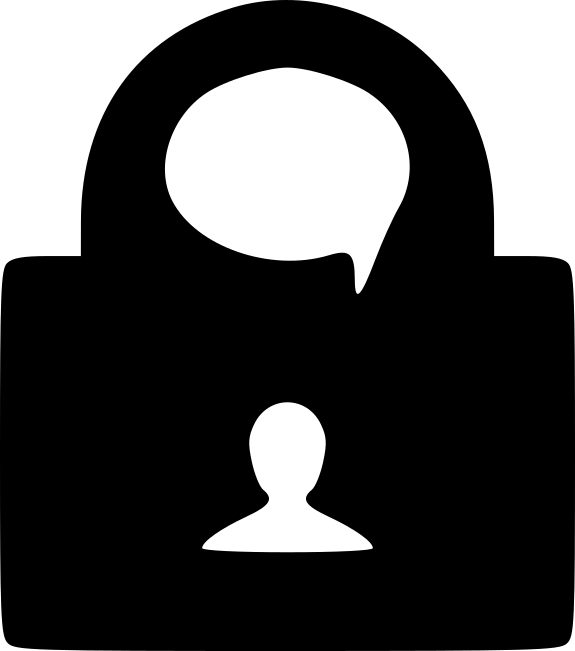
\includegraphics[width = 0.8\textwidth]{lock_chat.png} 
\end{figure}
{\large Computer Science Tripos, Part II}\\ \vspace{3mm}
{\large St John's College} \\ \vspace{3mm}
{\large 13th May, 2016}
\vfill
\clearpage
\endgroup}

\setlength{\fboxsep}{1pt}
\setlength\parindent{0pt}

\begin{document}

\titleTH

\pagenumbering{roman} % Roman page numbering

\chapter*{Proforma}
\begin{tabular}{l >{\bfseries}l}
    Name: & Pavel Berkovich \\
    Title: & NoNaMe -- Peer-to-peer conversation security using KleeQ \\
    Examination: & Computer Science Tripos, Part II, June 2016 \\
    Approx. Word Count: & {\color{red} TODO} \\
    Project Originator: & Pavel Berkovich \\
    Project Supervisor: & Dr. Richard Clayton \\
    Special Difficulties: & None
\end{tabular}

\section*{Original Aims of the Project}
The aim of this project has been to produce an implementation of KleeQ, a peer-to-peer conversation security protocol designed for devices with limited connectivity, and evaluate its performance and practicality in the broader context of Internet messaging. The intention was to preserve the security guarantees of the original design as well as understand its limitations that could potentially be used as attack vectors. It was also expected that a useable prototype of a messaging application would be produced, to evaluate the usability implications of the design as well as demonstrate the work of the implementation.

\section*{Summary of the Work Completed}

Each of the project's aims has been successfully achieved. Despite it taking more time than expected, the protocol has been implemented in full, according to the specification, retaining all of the security properties of the design. The implementation has demonstrated some impressive performance characteristics, highlighting some of the practical benefits that the use of the protocol can offer. A prototype of a messaging system, comprising a client application as well as some external components, has been implemented and tested. \\

{\color{red} 
Re-write with more specific results (with numbers etc) after do eval???}

\pagebreak
\section*{Declaration of Originality}
I Pavel Berkovich of St John's College, being a candidate for Part II of the Computer Science Tripos, hereby declare that this dissertation and the work described in it are my own work, unaided except as may be specified below, and that the dissertation does not contain material that has already been used to any substantial extent for a comparable purpose. \\[0.8cm]
\begin{tabular}{l}
    Signed \\[0.8cm]
    Date
\end{tabular}
\vfill

\tableofcontents

\skippage

\pagenumbering{arabic} % Arabic page numbering
\pagestyle{headings}

\chapter{Introduction}
\label{ch:intro}

\section{Overview of Secure Messaging}
\label{sec:intro.overview_sec_mess}
The era of global communication has presented humanity with many opportunities, but has also made our private lives more vulnerable to intrusion. Given the broad range of cyber-threats that our society is facing today, there is now significant demand for secure communication systems. The recent disclosures about widespread state surveillance programmes demonstrated the massive scale of the resources that a potential adversary might posses, and lead to fundamental change in public perception of what security means. As a result, we are now witnessing an unprecedented level of effort to develop messaging systems emphasising security and privacy. Some of these systems enjoyed considerable popularity whilst others remained largely unknown to non-experts, but each of them has been found to have some security flaws\footnote{\url{https://www.eff.org/secure-messaging-scorecard}} or usability problems.\\

Discussing secure messaging in more detail and comparing different solutions requires a clearly defined threat model and a systematic evaluation framework. One possible approach was proposed by Unger et al~\cite{unger2015sok} in a recent survey of the existing secure messaging systems which identified three key problems that any secure messenger must solve, namely:

% It is worth pointing out that, similarly to many other information security products, secure chats present an example of what is known as a ``market for lemons'' \cite{akerlof1970lemons} \cite{anderson2001information}. In this type of market, buyers have no feasible way to assess the quality of what is offered, and success of a product is determined by other factors (e.g. low price, short time-to-market), leaving producers with no economic incentive to invest in developing high-quality solutions. For secure chats, this implies that commercial success of a messaging application is by no means a measure of its actual security. \\ 

\begin{description}[labelindent=0.5cm, leftmargin=1.3cm, rightmargin=0.5cm]
    \item[Problem 1: Trust Establishment]\hfill \\
        How do we know that our peers are who they say they are? How do we make sure that they are not being impersonated by a malicious adversary?
    \item[Problem 2: Conversation Security]\hfill \\
        Once we are sure that we are talking to the right parties, how do we protect the security and privacy of the \emph{conversation's content}? In other words, how do we encrypt the messages, what data do we attach to them, and what security protocols do we perform?
    \item[Problem 3: Transport Privacy]\hfill \\
        Once we have secured the content of our messages, how do we actually \emph{send} them so as to \emph{hide their metadata} (e.g. sender identity, recipient identity, conversation to which the message belongs etc)?
\end{description}
The area of focus for this project is \emph{conversation security} (Problem 2 above).

\section{Aims of the Project}
\label{sec:intro.aims}
This project aims to build on KleeQ \cite{reardon2007kleeq} -- a peer-to-peer conversation security protocol that protects the content of conversation in a fully connected group (clique) of trusted participants communicating in a broadcast manner. \\

The scheme relies on Diffie-Hellman key exchange for deriving a common key which is used for encryption and message authentication. Protocol uses the \emph{patching algorithm} to exchange messages and converge on a global transcript. To ensure integrity of the conversation, the transcript is then verified in blocks of several messages via the process of \emph{sealing}. KleeQ achieves forward and backward secrecy by asynchronously rotating keys after a block is sealed, meaning that a compromised key only gives the adversary the ability to read messages within one block, but not in the previous or subsequent ones. The protocol enables users to repudiate authorship of specific messages as well as participation in a given conversation, since it only uses the common keys derived as part of the conversation to authenticate messages and makes no use of public keys. The asynchronous nature of the protocol makes it resilient to unstable network conditions and makes it possible to write messages while offline and then re-converge on a single transcript when connection is re-established. \\

As compared to other conversation security solutions \cite{unger2015sok}, KleeQ finds a good balance between security and usability characteristics which makes it a promising candidate for use in general-purpose messaging applications. \\

The authors of KleeQ (Reardon et al, \cite{reardon2007kleeq}) omitted some details in the protocol's description and only provided an unstable proof-of-concept implementation. This project aims to take their work further by re-implementing KleeQ from scratch preserving all of its security guarantees, and evaluating its performance and practicality for use in everyday messaging. More specifically, the objectives are as follows:

\begin{description}[labelindent=0.5cm, leftmargin=1.3cm, rightmargin=0.5cm]
    \item[Implementation] \hfill \\
        Fill out the gaps in the protocol's description and construct a messaging application based on it, preserving the security features of the original design.
        
    \item[Evaluation of Performance] \hfill \\
        Use the newly created application to evaluate the performance of the protocol and determine what limits it would impose on potential deployment.
        
    \item[Evaluation of Usability] \hfill \\
        Understand the usability implications of the protocol and assess the feasibility of its use in different kinds of consumer messaging systems.

\end{description}

%The area of focus for this project is \emph{conversation security} (\cref{ssec:convsec}), which is concerned with protecting the \emph{content} of messages from the adversary. The project involves implementing and evaluating KleeQ \cite{reardon2007kleeq} -- a peer-to-peer conversation security protocol with the following security guarantees:
%\begin{description}[labelindent=0.5cm, leftmargin=1.3cm]
%    \item[Confidentiality] \hfill \\
%        Nobody except the conversation participants can read the messages.
%    \item[Intergrity of conversation] \hfill \\
%        The adversary cannot inject, modify or replay messages.
%    \item[Forward secrecy] \hfill \\
%        A compromised key does not enable reading of previously encrypted messages.
%    \item[Backward secrecy] \hfill \\
%        A compromised key does not enable reading of subsequently encrypted messages.
%    \item[Authorship repudiation] \hfill \\
%        Given the transcript of a conversation and access to all keys, there is no computationally feasible way to prove that a given message was written by a particular participant.
%    \item[Participation repudiation] \hfill \\
%        Given the transcript of a conversation and access to all keys except for one user, there is no computationally feasible way to prove that this user was in a conversation with any of the others.
%\end{description}
%
%The above guarantees make KleeQ one of the most secure protocols to date. At the same time, it has some convenient usability characteristics, for example:
%\begin{description}[labelindent=0.5cm, leftmargin=1.3cm]
%    \item[Support for groups] \hfill \\
%        Unlike many other solutions, KleeQ supports group communication natively.
%    \item[Peer-to-peer (P2P)] \hfill \\
%        The protocol is peer-to-peer, so no additional service provider is required.
%    \item[Support for asynchrony] \hfill \\
%        It is possible to send messages to disconnected peers, to be delivered when they go back online again.
%    \item[Unreliable network resilience] \hfill \\
%        The protocol was originally proposed for devices with transient connectivity, so it assumes that the network can delay, drop or re-order messages.
%\end{description}
%
%Whilst having an unconventional design, KleeQ strikes a good balance between security characteristics and usability, which seems to be the key trade-off in secure messaging at the moment. \\
%
%The authors of KleeQ (Reardon et al, \cite{reardon2007kleeq}) described the core components of the protocol in sufficient detail, but only provided an unstable proof-of-concept implementation in Python. This project aims to build on their work, with the objectives summarised as follows:
%\begin{description}[labelindent=0.5cm, leftmargin=1.3cm]
%    \item[Implementation] \hfill \\
%        Fill out the gaps in the protocol's description and construct a more robust implementation in Java, preserving the security features of the original design.
%        
%    \item[Evaluation of Performance] \hfill \\
%        Use the newly created implementation to evaluate the performance of the protocol and its practicality for use in ubiquitous secure messaging.
%        
%    \item[Evaluation of Security] \hfill \\
%        Understand the limitations of the protocol. See what further work would need to be done to eliminate the remaining attack vectors.
%        
%    \item[Messenger Prototype] \hfill \\
%        Build a prototype of a messaging application based on KleeQ, with the view to assess the usability implications of the protocol.
%\end{description}

\section{Summary}
This chapter has shown where this project fits in the field of secure messaging, and described the objectives it expects to meet. The specifics of how these objectives are addressed are described in the following chapters.

\chapter{Preparation}
\label{ch:prep}

\section{Protocol Description}
\label{sec:prep.proto}

\subsection{Assumptions}
KleeQ takes its name from the word ``clique'', which is a graph-theoretic term for a fully connected graph (Figure \ref{fig:clique}).
\begin{figure}[h]
    \centering
    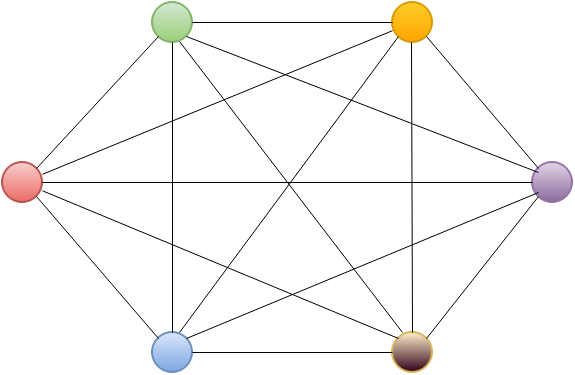
\includegraphics[scale = 0.5]{pics/clique.png}
    \caption{Clique of size $n = 6$ \label{fig:clique}}
\end{figure}
The protocol assumes that conversation participants form a clique (i.e. no two of them are strangers) and that all clique members are trustworthy (i.e. that the problem of Trust Establishment from \cref{sec:intro.overview_sec_mess} has already been solved via other means). 


\subsection{Clique formation}
Every clique has a \emph{common secret} that all participants share and which is regularly updated. When a clique is started, members are added one-by-one. One of the members first creates a singleton clique with a random secret, and then adds other participants. To add a user, one of the clique members performs a Diffie-Hellman key exchange \cite{diffie1976new} with the them, using the current clique secret as the secret exponent, thereby negotiating a new common secret based on the previous one. When other clique members are notified of the new user, they also update their version of the secret. 

Diffie-Hellman is a key exchange protocol that allows two parties to establish a common secret over an insecure channel. It uses two fixed publicly known parameters $G$ and $P$, such that $G$ is a generator of the cyclic group of order $P$. Let's say user Alice is a member of an existing clique with common secret $s$, and she wants to invite user Bob to the conversation. 
\begin{figure}[h]
    \captionsetup{width=0.8\textwidth}
    \centering
    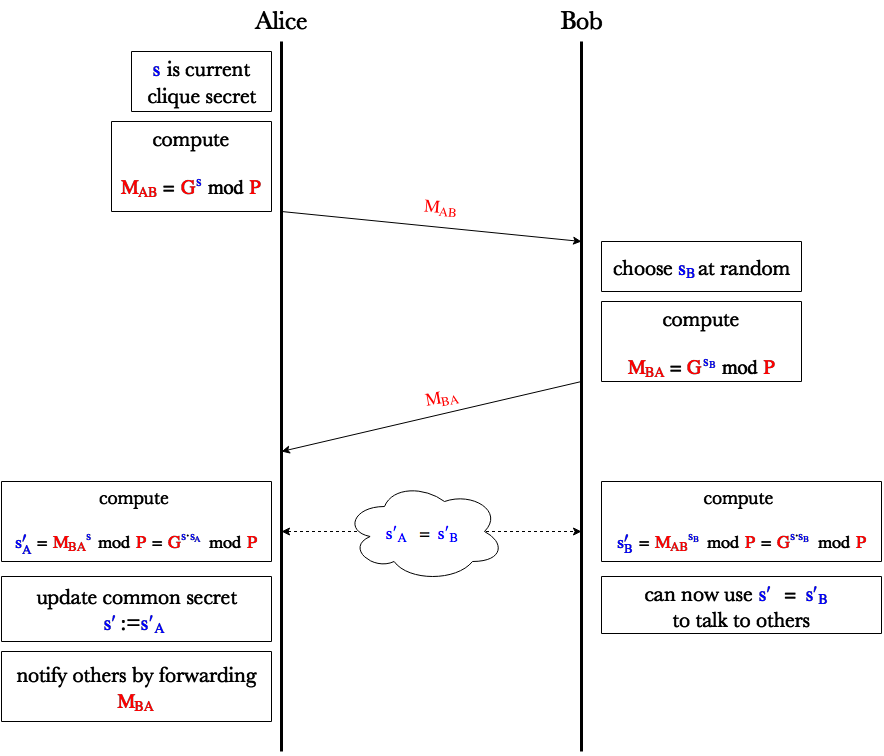
\includegraphics[width = 0.85 \linewidth]{pics/DH.png}
    \caption{Adding a new user to an existing clique using Diffie-Hellman key exchange. Public information is in {\color{red}red}, secret -- in {\color{blue}blue}.}
    \label{fig:DH}
\end{figure}

She sends Bob the modular exponent $M_{AB} = G^{s} \bmod P$. Upon receiving this message, Bob generates a random number $s_B$ and sends Alice $M_{BA} = G^{s_B} \bmod P$. Bob now computes $s'_B = M_{AB}^{s_B} \bmod P = G^{s \cdot s_B} \bmod P$. When Alice receives Bob's response, she computes $s'_A = M_{BA}^{s} \bmod P = G^{s \cdot s_B} \bmod P$ and updates the clique's common secret to be this new value. Clearly, $s'_A = s'_B = s'$, so Bob now also knows the secret and can use it to participate in the conversation. \\

An adversary who can observe this exchange and see both $M_{AB}$ and $M_{BA}$ has no computationally feasible way to determine the values of $s$ and $s_B$ and cannot compute the common secret $s' = G^{s \cdot s_B}$. The security of Diffie-Hellman relies on the difficulty of the Discrete Logarithm Problem in the chosen cyclic group, so it makes sense to choose parameters $G$ and $P$ to be very large. It is also worth pointing out  that this scheme is clearly vulnerable to a man-in-the-middle attack where an active adversary modifies the values of $M_{AB}$ and $M_{BA}$, essentially impersonating each user to the other one. This can be solved by some form of authentication, but this problem belongs to the realm of Trust Establishment (\cref{sec:intro.overview_sec_mess}) and is therefore outside the scope of KleeQ.


\subsection{Exchanging messages}
Clique members exchange messages through the procedure of \emph{patching}. This process needs two pieces of information that each user maintains -- the current \emph{transcript} of the conversation and the \emph{version vector}. The version vector is a vector of same size as the clique, where each entry corresponds to the number of messages authored by a particular conversation participant. The \emph{patching algorithm} is then as follows: \\ 
\begin{algorithm}
\caption{The Patching Algorithm}
\label{alg:patching}
{\bfseries Alice}
\begin{enumerate}
    \item Sends her version vector $v_A = (v_{A1}, v_{A2}, ..., v_{An})$ to Bob. \\
\end{enumerate}

{\bfseries Bob}
\begin{enumerate}
    \item Calculates the difference between his own version vector and the one sent by Alice, to see what messages she is missing:
        \begin{equation*}
            v_{\Delta} = v_B - v_A
        \end{equation*}
    \item {Generate a patch to provide the missing messages: \newline \vspace{-5mm}}
        \begin{algorithmic}
            \STATE \textit{Patch} $\leftarrow \emptyset$
            \FOR{$i$ from $1$ to $n$}
                \IF{$v_{\Delta i} > 0$}
                    \STATE \textit{Patch.add}(last $v_{\Delta i}$ messages authored by participant $i$)                        
                \ENDIF
            \ENDFOR
        \end{algorithmic}
    \item Send the \textit{Patch} and version vector $v_B$ to Alice. \\
\end{enumerate}

{\bfseries Alice}
\begin{enumerate}
    \item Insert the messages provided by Bob into transcript.
    \item As above, compute difference between $v_A$ and $v_B$, to see what messages Bob is missing.
    \item As above, generate a \textit{Patch} and send it to Bob. \\
\end{enumerate}

{\bfseries Bob}
\begin{enumerate}
    \item Insert the messages provided by Alice into transcript.
\end{enumerate}
\end{algorithm}

The above exchange happens regularly between every pair of clique members, and makes sure that their views of the transcript contain the same messages. \\

In order to ensure identical \emph{ordering} of messages in the clique, each participant also maintains a \emph{Lamport timestamp} which is initially set to 0. When two users patch each other as shown above, they update their timestamps to one plus the maximum of their Lamport times. Every time a message is written, it is given the current Lamport time of the author which is then incremented by one. We can thus define a \emph{total order} $<_L$ on messages as follows:

\[
    <_L(m_1, m_2) = 
        \begin{cases}
            \mathtt{TS}(m_1) < \mathtt{TS}(m_2) & \mathtt{TS}(m_1) \neq \mathtt{TS}(m_2) \\
            <_{lex}(\mathtt{Author}(m_1), \mathtt{Author}(m_2)) & \text{otherwise}
        \end{cases}
\]

where $\mathtt{TS}$ is the Lamport timestamp of a message and $<_{lex}$ is lexicographic comparison of authors' names. The $<_L$ relation allows the clique members to arrange all messages in a linear sequence, sorting them by Lamport time and breaking ties by comparing the names of authors lexicographically. \\ 

It can be formally proven \cite{reardon2007kleeq} that exchanging messages as specified by Algorithm \ref{alg:patching} and ordering them using the $<_L$ relation results in all participants converging on the same version of the transcript.


\subsection{Transcript verification}
In an ideal situation, just using the scheme above will allow the clique to converge on a single transcript. However, in the more realistic setting where network errors can occur or a malicious adversary can try to inject fake content, measures must be taken to verify the \emph{integrity} of the conversation. In other words, it is necessary to make sure that all users have the same view of the conversation. This is done using the process of \emph{block sealing}. \\

In brief, the scheme involves the clique members independently dividing the transcript into blocks in a deterministic fashion and \emph{sealing} them by comparing the hashes of their content. For this to work, it is necessary to choose blocks to be sealed in a way which would guarantee that there are no missing messages in them. This task is performed by the \emph{block sealing algorithm} (Algorithm \ref{alg:block_find}).



\begin{algorithm}
\caption{The Block Finding Algorithm}
\label{alg:block_find}
\textbf{Input}
\begin{itemize}
    \item $C$: clique
    \item $M$: sequence of unsealed messages (\emph{tail}) \\
\end{itemize}

\textbf{Output}
\begin{itemize}
    \item $B$: prefix of $M$ which is a sealable block, or $\emptyset$ if no such block can be found \\
\end{itemize}

\textbf{Variables}
\begin{itemize}
    \item SeenSet: set of uniquely seen authors
\end{itemize}


\textbf{Procedure}
\vspace{3mm}
\begin{algorithmic}
    \STATE Stage 1: calculate the sealable set \vspace{3mm}
    \STATE
    \begin{enumerate}
            \STATE SeenSet $\leftarrow \emptyset$
            \begin{spacing}{1.2}
            \FOR{$i$ from $|M|$ down to $1$}
                \STATE $m \leftarrow M[i]$
                \STATE $SeenSet \leftarrow SeenSet \cup \{Author(m)\}$
                \IF{$|SeenSet| = |C|$}
                    \STATE $S \leftarrow M[1..i]$
                    \STATE \textbf{break}
                \ENDIF
            \ENDFOR
            \IF{$|SeenSet| \neq |C|$}
                \RETURN $\emptyset$
            \ENDIF
            \end{spacing}    
    \end{enumerate}
    \STATE \textbf{Stage 2: computing the sealable block \vspace{3mm}}
    \begin{enumerate} \setcounter{enumi}{3}
        \STATE SeenSet $\leftarrow \emptyset$
        \begin{spacing}{1.2}
        \FOR{$i$ from $1$ up to $|S|$}
            \STATE $m \leftarrow S[i]$
            \STATE $SeenSet \leftarrow SeenSet \cup \{Author(m)\}$
            \IF{$|SeenSet| = |C|$}
                \RETURN $S[1..i]$
            \ENDIF
        \ENDFOR
        \end{spacing}
        \vspace{-2mm}
        \RETURN $\emptyset$
    \end{enumerate}

\end{algorithmic}





\end{algorithm}


\subsection{Key management}

\section{Requirements Analysis}

\section{Preliminary System Design}

\section{Implementation Strategy}

\section{Libraries and Tools}

\section{Summary}




\chapter{Implementation}


\chapter{Evaluation}


\chapter{Conclusions}



\bibliographystyle{unsrt}
\bibliography{bibliography}
\addcontentsline{toc}{chapter}{Bibliography}

\begin{appendices}
\chapter{Project Proposal}
\section{Introduction and Description of the Work}
\label{intro}
The recent public outcry in response to mass surveillance programs carried out by governments around the world led to creation of multiple messaging systems which emphasised security of communication. Some have been more successful than others, but each of them has been found to have some flaws or deficiencies. Broadly speaking, there are four problems that each security-oriented messenger needs to solve:
\begin{description}
    \item[Problem 1: Contact Discovery] \hfill \\
        How do we find out at which IP addresses our peers currently reside? How do we know where to send our messages?
    \item[Problem 2: Trust Establishment]\hfill \\
        Once we know where our peers are, how do we know that they are who they say they are? How do we make sure that they are not being impersonated by a malicious adversary?
    \item[Problem 3: Conversation Security]\hfill \\
        Once we are sure that we are talking to the right parties, how do we protect the security and privacy of the messages' content? In other words, how do we encrypt the messages, what data do we attach to them, and what security protocols do we perform?
    \item[Problem 4: Transport Privacy]\hfill \\
        What is the mechanics for actually sending the message so as to hide the message metadata (e.g. sender identity, recipient identity, conversation to which the message belongs etc).
\end{description}

\vspace{\baselineskip}
\noindent
Multiple protocols, with different threat definitions and varying levels of security, have been developed for each of these tasks. The aim of this project is to explore and build on KleeQ, one of the protocols aimed at providing conversation security (Problem 3 in the list above). Given a group of trusted parties residing at known addresses, it gives the following security guarantees for their conversation:
\begin{itemize}
    \item confidentiality of message content
    \item message integrity
    \item forward secrecy
    \item backward secrecy
    \item message authorship repudiation
    \item conversation participation repudiation
\end{itemize}
KleeQ has been designed for devices with transient connectivity (e.g. communication via Bluetooth or wireless), but the ideas introduced by this protocol can be used in the general setting of group messaging over a network.

\vspace{\baselineskip}
\noindent
In this project, KleeQ will be completely re-implemented into a general-purpose network conversation security protocol, preserving the security properties mentioned above. The performance characteristics will be tested, and the use of the protocol will be demonstrated by constructing a simple demo messaging app.

\vspace{\baselineskip}
\noindent
Optionally, if time allows, an attempt shall be made to make use of the most recent and secure third-party solutions to solve Problems 1, 2 and 4 from the list above, thereby producing a full-blown secure messaging application.


\section{Resources Required}
All the development will be based on the resources provided by my own machine and the PWF. In addition, it is expected that a commercial cloud hosting service (DigitalOcean, Heroku or similar) will be used, for the purpose of hosting the server side of the application. The backup strategy involves periodically pushing the code to a private GitHub repository and keeping a hand-written project log. No other resources will be required.


\section{Starting Point}
As of the starting date of the project, the following relevant background:
\begin{itemize}
    \item Experience of programming in Java, at the level of University courses \emph{Programming in Java} and \emph{Further Java}.
    \item Understanding of cryptographic primitives and computer security fundamentals, as taught in Part IB \emph{Security I} course.
    \item Limited experience of writing server-side code in Python using Flask.
\end{itemize}
\vspace{\baselineskip}


\noindent
The successful completion of the core part of the project will require the following:
\begin{itemize}
    \item Learning about the fundamentals of conversation security, understanding what security properties it entails and what the common attack strategies are.
    \item Understanding the algorithms and data structures introduced by KleeQ.
    \item Learning to write security-oriented code in Java.
\end{itemize}

\noindent
To complete the optional part, the following will need to be done:
\begin{itemize}
    \item Understanding the most common attack strategies employed by adversaries against secure messengers.
    \item Reading research papers and technical documentation describing the APIs presented by the third-party libraries in use.
\end{itemize}


\section{Substance and Structure of the Project}
\subsection{Core Part}
The core part of the project will involve re-implementing KleeQ, to make it a universal conversation security protocol. Initially, it will be necessary to obtain a deep understanding of how KleeQ operates which will be done by reading the relevant research material, as well as studying the source code of the current implementation. Then, the parts of the protocol which require re-designing to allow network communication (as opposed to ad-hoc communication via Bluetooth or similar) will be identified, and the necessary design decisions will be made. The next step will be implementing the protocol in Java and testing it locally. At that point, additional checks will be made to ensure that the new implementation retains all the security properties of the original one and, if necessary, eliminate the possible loopholes in the code.

\vspace{\baselineskip}
\noindent
The next step will be turning the result of the above into a simple desktop P2P messaging application. It is important to understand that producing a full-blown secure messaging system is outside the scope of the core part of this project -- at this stage, the aim will be to write some simple and not necessarily secure "scaffolding" code to produce a prototype, for the purposes of demonstrating the work of the new protocol implementation. In particular, it is expected that a minimalistic graphical user interface and a simple server-based contact discovery component will be implemented at this point.


\subsection{Optional Extensions}
If time allows, the most recent and secure approaches may be used to convert the aforementioned demo application into a proper secure messaging system. As mentioned in Section \ref{intro}, this would require solving the problems of secure contact discovery, trust establishment and transport privacy. These problems can be solved in the following ways:
\begin{itemize}
    \item DHT with query anonymisation for contact discovery
    \item self-auditable public key logs for trust establishment (using CONIKS)
    \item Tor-based hidden service for transport privacy and metadata hiding
\end{itemize}
All of the above are available in the form of open-source libraries which can be used in the project without major modifications.

\vspace{\baselineskip}
\noindent
In addition, an effort may be made to improve the usability of the application. With this in mind, the GUI will be refined to match the usability of the most ubiquitous messenger applications (e.g. WhatsApp, Viber, Telegram etc).




\section{Success Criteria}
There shall be two measures of success for this project:
\begin{enumerate}
    \item Implementation of a working messaging system which would be possible to use.
    \item Preservation of the security properties of the original KleeQ implementation, namely:
        \begin{itemize}
            \item confidentiality of message content
            \item message integrity
            \item forward secrecy
            \item backward secrecy
            \item message authorship repudiation
            \item conversation participation repudiation
        \end{itemize}
\end{enumerate}




\section{Timetable and Milestones}
It is important to structure the project in a way which would allow to evenly distribute the workload over the available time and minimise risks of missing deadlines. In addition, as pointed out by previous Part II students, it would be beneficial to finish the dissertation write-up at least two weeks in advance of the official deadline, to allow more time for Tripos revision. With this in mind, the following schedule has been set:


\subsection*{Weeks 1-2 (Oct 25 -- Nov 6)}
Do preliminary reading and understand the algorithms and data structures used by KleeQ, referring to the existing implementation as necessary. Identify the parts of the protocol which require modification, and design the object-oriented structure of the new implementation. Decide on which standard Java classes will need to be used. Find out what common implementation mistakes result is security loopholes. Arrange the necessary infrastructure, such as a back-up repository and cloud hosting space.

\vspace{0.7\baselineskip}
\noindent
\textit{Milestone:} The necessary knowledge of the protocol acquired, design and infrastructure ready -- can begin writing code.

\subsection*{Weeks 3-7 (Nov 7 -- Dec 11)}
Implement the protocol in Java. Test locally. Watch out for most common implementation vulnerabilities. Make sure the original security guarantees are in place.

\vspace{0.7\baselineskip}
\noindent
\textit{Milestone:} The conversation security protocol implemented and tested.

\subsection*{Weeks 9-10 (Dec 12 -- Dec 25)}
Turn the protocol implementation into a library which would be usable by third parties in their applications.

\subsection*{Week 11 (Dec 26 -- Jan 1)}
A week-long holiday is planned for these dates. No work will be done during this time.

\subsection*{Weeks 12-13 (Jan 2 -- Jan 15)}
Implement the "address book" server application to allow contact discovery. Make sure the server has the most current information about user's status. Test the practicality of KleeQ's conversation concepts.

\subsection*{Week 14 (Jan 16 -- Jan 22)}
Write-up the progress report and submit it one week ahead of the deadline.

\subsection*{Weeks 15-16 (Jan 23 -- Feb 5)}
Create a minimalistic GUI. Make sure that the cases of asynchrony (device going offline or coming back online) are adequately handled.

\vspace{0.7\baselineskip}
\noindent
\textit{Milestone:} An operational messaging application is ready. Core part of the project finished, the success criteria satisfied.


\subsection*{Weeks 17-19 (Feb 6 -- Feb 26)}
Evaluate how the protocol performs over a network under high load, and try to tune it to perform better. Refine the GUI of the prototype to allow usage by non-experts.

\vspace{0.7\baselineskip}
\noindent
\textit{Milestone:} The application looks good and the performance is satisfactory.

\subsection*{Weeks 20-21 (Feb 27 -- Mar 11)}
Implement the optional extensions as time allows. Make sure that none of the previously implemented security guarantees are broken.

\subsection*{Week 22 (Mar 12 -- Mar 18)}
A week-long holiday is planned for these dates. No work will be done during this time.

\subsection*{Weeks 23-27 (Mar 19 -- Apr 22)}
Write up the dissertation. Use the project log to recollect the details of what work has been done and how. Pay special attention to the Evaluation section, describing in detail the previously made performance measurements. Arrange regular meetings with the supervisor to receive feedback and iteratively refine the work. This part of work will take a long time, since it will be interleaved with Tripos revision over the Easter Vacation.

\vspace{0.7\baselineskip}
\noindent
\textit{Milestone:} Dissertation largely written. The supervisor and the overseers are satisfied with the content.

\subsection*{Weeks 28-29 (Apr 23 -- May 13)}
No project work is scheduled for these days -- the intention is to use this time for Tripos revision. It also provides a "safety buffer" in case more time is required, for one reason or another. If necessary, final adjustments to the text of the dissertation will be made at this time.

\vspace{0.7\baselineskip}
\noindent
\textit{Milestone:} Dissertation printed, bound and submitted at least two weeks ahead of the deadline.
\end{appendices}



\end{document}
